\documentclass{article}
\usepackage{graphicx}  % Include the graphicx package
\usepackage{ifxetex,ifluatex}
\usepackage{bookmark}
\usepackage{cite}
\usepackage{adjustbox}
\usepackage{amsmath}
\usepackage{hyperref}
\usepackage{graphicx}
\usepackage{float}
\usepackage[a4paper, top=3cm, bottom=3cm, left=3cm, right=3cm]{geometry}

\begin{document}

\title{
  \vspace{-3cm}  % Adjust vertical space before the images
  \begin{minipage}{0.48\textwidth}
     \raggedright  % Aligne at the left
    
\includegraphics[width=0.6\textwidth]{images.png}  % First image on the left
   \vspace{2cm}
  \end{minipage}
  \begin{minipage}{0.48\textwidth}
    \raggedleft
 
    
\includegraphics[width=0.6\textwidth]{lepmi_logo.png}
    \vspace{2cm}
    % Second image on the right
  \end{minipage}
  \vspace{2cm}

  \textbf{\Large Influence of KCl and NaCl Proportions in\\
  ${Li(Ni}_{0.8}{Co}_{0.1}{Mn}_{0.1}{)O}_{2}$ }\\ 
  \vspace{0.3cm}
  \textbf{\Large Molten Salt Synthesis for Li-ion Batteries}
    \vspace{4cm}
  }
 

\author{
  \textbf{Authors}\\
  Noriega Franco Santiago \\
  Choppe Apolline \\
  Brétillon Laura\\
  \\
  \textbf{Supervisors}\\
  Eddy Coron\\
  Julia Levy\\
  Lenka Svecova}


\date{
  \vspace{2cm}
  \small{January 24, 2024}
}




\maketitle
\newpage
\setcounter{page}{1}  % Start counting from 1
\tableofcontents

\newpage
\section{Abstract}
\section {Introduction}

\subsection{Context}

Lithium-ion batteries are a key technological tool for the sustainable mobility development all around the world. The performance of these batteries are highly influenced by the materials composition, morphology, crystal structure and synthesis parameters, specially for the positive electrode material and the electrolyte.\cite{topo} \\

NMC (Nickel-Manganese-Cobalt oxide) is todays the predominant material used for the positive electrode in modern electric vehicle batteries. Current developments focus on reducing cobalt content in favor of increasing nickel in the structure, specifically transitioning towards high-nickel compositions such as NMC811. This shift aims to enhance energy density, lower material costs, and address ethical and environmental concerns associated with cobalt mining. \cite{NMC811} \cite{NMCintro} \\

The specific theoretical capacity calculated with Faraday law:

\begin{equation}
Q_{th} = \frac{n F}{3.6 M} 
\end{equation}

where n: number of electrons;
Faraday constant F = 96500 C/mol;
M=96.5 mol/g mass molar of NMC811;

\begin{center}
  

\begin{tabular}{|c|c|c|}
  
  \hline
  Specific capacity
theoretical
(mAh/g) & 280  \\
  \hline
  Average Voltage in discharge (V) & 3.7  \\
  \hline
\end{tabular}
\end{center}

However, the higher nickel content introduces significant challenges. Nickel's tendency to occupy lithium sites, a phenomenon known as cation mixing or positive electrode mixing, can degrade the crystal structure. This defect reduces lithium mobility, diminishes cycling stability, and impairs the battery's long-term performance. Furthermore, high-nickel NMC materials are more chemically reactive, which can lead to thermal instability and increased side reactions with the electrolyte.\cite{NMCintro} \\

Currently, there is a great need to avoid any waste form industry,
specially if you are working with scarce materials. The European Critical Raw Materials Act describes lithium, nickel and cobalt as crucial for the economy and asks for the implementation of a sustainable independent supply chain.\cite{RMA} Therefore some efforts
have been done to repurpose the waste of Li-ion batteries plants and turn them into a usable material. This project, attached to LEPMI laboratory and VERKOR, aims to repurpose byproduct carbonates (\({MnCO}_{3}\), \({CoCO}_{3}\) and \({NiOH}_{a}{({CO}_{3})}_{b}\) ) for the synthesis of NMC811 using a molten salt-assisted solid-state sintering method. \\


\subsection{Close-up on the Molten Salts Method}

\subsubsection{A Less Energy-Intensive Method}
Traditional synthesis methods for NMC require temperatures exceeding 900°C, resulting in high energy consumption. One alternative to this is the introduction of a liquid diffusion medium into the process. The presence of a liquid phase during calcination accelerates the overall reaction kinetics, acting as a more efficient medium for particle growth and homogenization. Once the process is completed and the material has solidified, the liquid phase is no longer needed, as it could interfere with the purity of the target material. For this reason, molten salts are used. These salts can easily dissolve in water, allowing them to be washed away, ensuring the purity of the synthesized material after processing.\cite{Heuristics}

\subsubsection{Choice of Salts}
The requirements for the salt selection were the following:
\begin {itemize}
\item Low melting point: The salt melting point needs to be adequate 
for the synthesis methodology and parameters. This also depends on the material
that is wanted to be synthesized.
\item Chemical inertness: The salt should not react with the other substances in the mixture. 
Another important consideration is that the solvated ions of the salt should not take lithium sites on 
the electrode's crystal structure.
\item Cost Effectiveness. The economic viability of the salt is also an important factor to consider.
specially if the process is wanted for industrial applications. 
\end{itemize}

\subsubsection{Single-crystal (SC) particles formation interest}

The \textbf{molten salt synthesis} method is a technique producing single-crystal particles, unlike the polycrystalline particles typically obtained through the solid-state method. Using molten salts, which act as a reactive medium at high temperatures. In their liquid state, these salts provide an environment that enables free ion movement, facilitating controlled crystal growth. This process allows the formation of single-crystal particles by favorating uniform growth and minimizing the formation of grain boundaries that are characteristic of polycrystalline structures. \cite{SC}
\\

This phenomenon is more precisely known as \textbf{Ostwald ripening} \cite{oswald}, which plays a crucial role in the formation and growth of particles. When a mixture of particles of varying sizes is heated in the molten salts, smaller particles, which are thermodynamically less stable due to their higher surface energy, tend to dissolve. The ions released from these smaller particles migrate through the molten salt medium and redeposit onto larger particles, which are more stable because of their lower specific surface area. This process, enhanced by the high ionic mobility in molten salts, leads to a reduction in particle size dispersion and a gradual increase in average particle size. Over time, the smaller particles disappear entirely, leaving only the larger ones, which develop into well-defined single crystals.\cite{moltensalt1}

Controlling the salt temperature and heating duration is crucial for tuning the final particle size. Higher temperatures and longer heating times accelerate the ripening process, resulting in larger particles. This precise control makes the molten salt method particularly advantageous to control size and morphology particles. \cite{moltensalt1} \\

The focus of this study is to synthesize using this method as well as to evaluate how different proportions of NaCl and KCl in the salt mixture affect the final product (morphology, composition, purety) and to analyze the electrochemical performance of the NMC positive electrode material.\cite{meltingp}The morphology and performance of NMC 811 for lithium-ion technologies will be analyzed using characterization techniques: Scanning Electron Microscopy (SEM), X-Ray Diffraction spectroscpoy to identify the material phases as well as electrochemical characterization techniques on coin cells: Charge/discharge protocol. \\
\section{State of Art}

\subsection{Positive electrode materials}

Todays positive electrodes are mostly intercalation or composite electrodes, they consist in a solid network that can host lithium ions with intercalation during discharge and deintercalation during discharge.
These compounds can be devided into several different structures; layered, olivine and spinel. \cite{topo} \\

Some common cathode materials in lithium-ions technologies are:
\begin{description}
 \subsubsection{Layered structures}
  \item[$\text{LiCoO}_{2}$]  (LCO). This material has low capacity compared to the theoretical one the extraction of more than half the lithium content leads to structural instabilities. It's use is also restricted due to the high cost of cobalt and its scarcity. \cite{topo}\cite{LCO}
 
  \item[$ \text{Li(Ni}_{0.8}\text{Co}_{0.1}\text{Mn}_{0.1}\text{)O}_{2} $]  (NMC811). NMC811 has more nickel and less cobalt than NMC111, which is better for the environment by reducing reliance on cobalt. However, this higher nickel content makes NMC811 batteries less stable and more prone to degradation and overheating compared to NMC111.\cite{topo}
  

  \item[$\text{LiNi}_{0.8}\text{Co}_{0.15}\text{Al}_{0.05}\text{O}_{2}$] (NCA).
  This material increases the charge capacity by changing the Co content with Ni and using aluminum as 
  a stabilizer. This reduces slightly the average cell voltage
  compared to LCO.\cite{topo}
\end{description}

\begin{description}
 \subsubsection{Spinel structures}
  \item[$\text{LiMn}_{2}\text{O}_{4}$](LMO).The specific lattice structure
  of LMO, allows diffusion on three dimensions, which leads to faster charge
  - discharge rates. It is also a greener solution compared to to 
  Co based positive electrode materials. The disadvantage of LMO is t
its low charge retention and low cyclability.\cite{topo}
\end{description}

\begin{description}
  \subsubsection{Olivine structures}
  \item[$\text{LiFePO}_{4}$](LFP). This is also a greener material than the 
  Co based structures. LFP has a really high thermal stability but only counts
  with one dimensional diffusion. Therefore the voltage of discharge
  is too low.\cite{Olivine} \\
\end{description}

\subsection{Synthesis methods}
The choice of synthesis method plays a critical role in determining the final properties of NMC materials. Key attributes such as tap density, particle size distribution, particle morphology (both primary and secondary shapes), and crystallinity are strongly influenced by the synthesis process. Additionally, the method chosen impacts the presence of impurities, the overall quality of the final product, and its electrochemical performance. \\

Various synthesis methods are available for producing NMC, including co-precipitation, solid-state reaction, sol-gel processes, hydrothermal methods, and spray pyrolysis \cite{process}. 

Each approach has its own advantages and limitations, influencing the structure and performance of the material in different ways. Below is an overview of the most commonly used methods for NMC synthesis:
\subsubsection{Co-precipitation}
This is today the most popular and cost effective production method, on an industrial scale
. The method consists on the simultaneous precipitation of the transition metals and a subsequent sintering with
a lithium source. The parameters important for this process is the pH of the solution, the stirring rate 
and the used chealing agent this highly affects the particle size and morphology. \cite{process}  \\
There are three types of co-precipitation depending on the precursors used;
\begin{itemize}
  \item Carbonate co-precipitation: This type of precipitation doesn't need an inert atmosphere
  because the oxidation state of the metals can be stabilized by CO. The problem is that
the control of the final morphology is limited. \cite{process}
  \item Hydroxide co-precipitation: The final product of this process is really
  cost effective and has high tap density. When sintered, the particle size doesn't change
  so much but it is possible to get impurities from manganese oxides.\cite{process}
  \item Oxalate co-precipitation: This method is considered more environmentally
  friendly than the other two, and even cheaper. It does not require an inert 
  atmosphere. The only problem is that the oxalate salts that are used 
  have low solubility in water, therefore the production rate would be lower\cite{process}.
\end{itemize}

\subsubsection{Sol-gel}
Sol-gel method is used on laboratory scale conditions. It consists on forming a gel from transition 
metal salts and a chealing agent that is then dried and sintered. It provides really good morphology and control over the stoichiometry\cite{process}.

\subsubsection{Solid state reaction}
This is one of the most classical methods to synthesize any kind of ceramic material. 
It consists on the correct mixing of the precursors, and then heating the powder below the fusion temperature of the material.
This activates the diffusion of the material due to surface energy phenomena, finishing on the coarsening of larger particles
in expense of smaller ones. The disadvantage of this method is the high dependence on the initial particle size distribution and 
the homogeneity of the mixture\cite{process}.

\subsubsection{Spray pyrolysis}
Spray Pyrolysis consists on atomizing the precursor in a solution at a really high temperature. This yields on a 
quite homogenous layer of mixed materials (not better that CVD or PVD). Here the properties depend on the solution concentration, the 
droplet size and the temperature of the process\cite{process}.

\subsection{Characterization methods}
There are several techniques to extract information from positive electrode materials,
these evaluate physical, chemical and electrochemical properties to evaluate the stability, morphology 
and performance of the material. Here is an overview of the characterization techniques used on this project.\\
\subsubsection{Scanning Electron Microscopy (SEM)}
This technique is useful to get high resolution imaging of the materials morphology.
It consists on a beam of electrons that scans the surface of the sample and the collection of three 
different signals; secondary electrons, backscattered electrons and X-rays. With the primary electrons 
being the ones emitted by the source.\\
\begin {itemize}
\item Backscattered electrons: These electrons are the ones that interact with the materials atoms and get back to
the sensor, the intensity of the signal can be related to the element's atomic mass. Heavier elements will scatter more electrons
to the sensor. Therefore, this signal is useful to get the composition and phases of the material.
The strength of this signal is also dependant on the topography of the samples surface, therefore a topographic image can be obtained.\\
\item Secondary electrons: The secondary electrons are the ones that interact in an inelastic way with the material, therefore they arrive to
the sensor with less energy. This signal is useful to get the morphology of the material because only the electrons that interact with the surface
are collected. The energy when collected is related to the surface morphology and an image is created.\\
\item X-rays: Are a byproduct generated when a primary electron removes an electron from the inner shell of an atom. The energy of the X-ray is related to the
atomic number of the element. This signal is useful for the creation of composition maps overlaying the 
SEM images.\\
\end{itemize}

\subsubsection{X-Ray Diffraction (XRD)}
X-Ray Diffraction is a non destructive technique used to characterize crystalline materials. 
It provides information about the crystal phases, structural parameters (ize of crystals, crystallinity  and defects) and the orientation of the crystals.\\
This method works by comparing the of the xray beam (with a wavelength $\lambda$) and the lattice planes called $\theta$. The reflected beam has an angle of $2\theta$, and this is the one that is measured.


\begin{equation}
2d \sin(\theta) = n\lambda   
\end{equation}

The Bragg's law is used to calculate the distance between the lattice planes (d), characteristic of the crystal structure. 
The intensity of the diffracted beam is related to the number of atoms in the crystal, the atomic number and the distance between the planes.\\

Today, databases can compare the diffraction spectra with the ones of known materials, to identify the phases present in the sample.\\

\subsubsection{Electrochemical characterization}

\subsection{Prior studies on Molten Salt Synthesis}
A prior study by the Karlsruhe Institute of Technology  worked on methods to 
synthesis of LNO using molten salts as a diffusive medium.
The aim of this study was to create a model for single crystal
layered lithium metal oxides (NCM's).\\
Here the molten salts as a tool to produce a single crystal
at relatively low temperatures.
The selected salts were NaCl, KCl, CsCl and \(K_{2}SO_{4}\), 
done at molar ratios to nickel from 1.0 to 4.0 \cite{meltingp}.\\
The results by SEM and XRD methods showed that the molar ratio
of the salts significantly affected the martials particle size with 
higher salt ratios, yielding in larger particles but not a special effect on the particle size distribution.
 The salt selection also affected the purity of the final sample \cite{meltingp}. \\
\section {Methodology} 
\subsection{NMC 811 electrode synthesis}

\subsubsection{Active material synthesis}

\textbf{Step 1: precursor mixing: }\\
Precursor mixtures were prepared with the stoichiometry of NMC811
 with excess lithium 15\%, and with the target of 4g of precursors. As three salt ratios are tested, three NMC precursors need to be made. Each species was weighted as stated in Table \ref{t1} in the three samples, and the salts were then added with different mass for each mixture according to Table \ref{t2}.
\begin{table}[h!]
    \centering
    \begin{tabular}{|c|c|}
        \hline
        \textbf{Species} & \textbf{Mass (g)} \\ 
        \hline
        MnCO$_3$ & 0.589 \\
        CoCO$_3$ & 0.610 \\
        Ni(OH)$_a$(CO$_3$)$_b$ & 4.508 \\
        LiOH & 2.828 \\
        \hline
    \end{tabular}
    \caption{Mass of each components used for NMC 811 synthesis other than the salts.}
    \label{t1}
    
\end{table}
\begin{table}[h!]
  \centering
  \begin{tabular}{|c|c|c|c|}
    \hline
    \textbf{Salt ratio (NaCl:KCl)} & \textbf{Mass of NaCl (g)} & \textbf{Mass of KCl (g)} & \textbf{Total mass (g)} \\ 
    \hline
    1:1 & 2.971 & 3.791 & 6.762 \\ 
    6:4 & 3.566 & 3.033 & 6.598 \\ 
    4:6 & 2.377 & 4.549 & 6.926 \\ 
    \hline
  \end{tabular}
  \caption{Masses of NaCl and KCl for different salt ratios used in NMC synthesis.}
  \label{t2}
\end{table}


\textbf{Step 2: Ball milling:}\\
Each sample is then mixed with ball milling, using 60 ZrO2 4.5mm beads in a 45 mL bowl air and 4 cycles of the following programme: rotations at 250 rpm during 5 min, then 10 min rest. \\

\textbf{Step 3: Pre-annealing:}\\
The three mixtures obtained are then heated at 500°C in an oven: first, a ramp of 5°C/min during 100 min to reach 500°C, then this temperature is held during 3h. This step aims to melt the LiOH in the precursors, as this Li-source melting point is 462°C. \cite{precalci} \\

\textbf{Step 4: Annealing:}\\
The pre-annealed samples are then calcinated in an oven at 800°C for 12h, after a ramp of ??. The salt mix melts, as its melting point is at 660°C, but not the NMC material as it melts above 800°C. When the samples are annealed, they are then cooled down naturally.\\

\textbf{Step 5: With or without ball milling:}\\
Each annealed NMC precursor are grounded in a morter and divided in two samples: an  A one and a B one, that will follow different protocols. The samples B have a additionnal ball milling step, with the same parameters as before: 4 cycles of rotations at 250 rpm during 5 min cut by 10 min rest, using 60 ZrO2 4.5mm beads in a 45 mL bowl air. The goal is to homogenize the grains again. As for samples A, they are not ball milled and go directly to the next step of the protocol.\\

\textbf{Step 6: Washing:}\\
Each one of the grounded or ball-milled NMC samples are then washed using vacuum filtration. The filters used are 47 mm Milipore Express PLUS 0.22µm PES Membrane, and the powder is added on top. It is rinced several times with distilled water to remove the salt from the NMC material, with approximately 250 mL of water in total. NaCl and KCl then dissolve in the water as  $Na^+, K^+$ and $ Cl^-$ and pass through the filter, leaving the NMC powder. The solid material is dried in the air after the washing, to remove the water. \\

\textbf{Step 7: Last annealing:}\\
After the washing step, the samples are once again heated in the oven, this time at 600°C for 3h with a prior ramp of ??. This last step of the NMC 811 materials synthesis aims to release the CO2 gas that can still remains in the powder, or even some carbonates. It is also a way to effectively dry the material previously washed.\\

\subsubsection{Ink preparation}
To make a functioning possitive electrode to be tested inside a coin cell, 
the NMC 811 obtained needs to be mixed with a conductive carbon and a binder into a slurry.
This mixture needs to be composed by 80\% of NMC 811, 10\% of conductive carbon and 10\% of binder.\\
Here, the carbon black is used as a conductive matrix, and helps create ionic paths for the electrolyte 
to fill the pores and have a good contact with the NMC 811\cite{Itou}. The binder is a polymer called polyvinylidene difluoride (PVDF),
is used to keep the material together.\\
NMP (N-Methyl-2-pyrrolidone) is used as the solvent to adjust the viscosity of the ink. It should be added gradually to avoid clumps. Cyclohexane can be added to improve dispersion of active material in the mixture, it evaporates quickly under the hood when heated to 80°C.\\
\textbf{Process of Ink Preparation:}\\
\begin{itemize}
  \item The NMC, carbon black and PVDF are weighted in the correct proportions that are represented on 
  table \ref{t3}.
  \item The materials are first mixed in a speed mixer (Hauschild SpeedMixer DAC 250.3 SP)  at 1500 rpm for 2 minutes to ensure all particles are coated. A second mixing step at 2500 rpm for 8 minutes, with additional NMP, is performed to achieve the desired consistency.
  \item The ink is then coated onto aluminum foil using an adjusted blade of 15 um. Proper ventilation must be ensured during the process, and the blade used for coating should be cleaned beforehand. Coating is performed at a low speed for uniform application. The desired wet thickness is 150 µm, which dries to 20-30 µm, when applied on aluminum.
  \item The electrode coating was dried in an oven for 12 hours, after which it was cut using a punch cutter. Three electrodes, each with a diameter of 12 mm, were then weighed to ensure consistent weight across samples, thereby maintaining the same active material mass.
  \begin{itemize}
    \item The NMC, carbon black and PVDF are weighted in the correct proportions that are represented on 
    table \ref{t3}.
    \item The materials are first mixed in a speed mixer (Hauschild SpeedMixer DAC 250.3 SP)  at 1500 rpm for 2 minutes to ensure all particles are coated. A second mixing step at 2500 rpm for 8 minutes, with additional NMP, is performed to achieve the desired consistency.
    \item The ink is then coated onto aluminum foil using an adjusted blade of 15 um. Proper ventilation must be ensured during the process, and the blade used for coating should be cleaned beforehand. Coating is performed at a low speed for uniform application. The desired wet thickness is 150 µm, which dries to 20-30 µm, when applied on aluminum.
    \item The electrode coating was dried in an oven for 12 hours, after which it was cut using a punch cutter. Three electrodes, each with a diameter of 12 mm, were then weighed to ensure consistent weight across samples, thereby maintaining the same active material mass.
    \begin{itemize}
      \item The active material mass (mg) was calculated as:\\
       Active material mass (mg) =  80\% \(\times\) total mass of NMC811.
    \end{itemize}
    \item The thickness of the coating was measured using a … . This measurement was used to calculate the coating volume and subsequently the porosity:\\
    \begin{center}
    Porosity (\%) = 100 \(\times\) (1 - \(\frac{Coating Volume }{Theoretical Volume }\))\\
    
  \end{center}
    Where the  coating volume is the thickness times tne area of the electrode. 
  \end{itemize}
  
\end{itemize}
\begin{table}[h!]
  \centering
  \begin{adjustbox}{width=1\textwidth}
  \small
  \begin{tabular}{|c|c|c|c|c|c|}
    \hline
    & \textbf{Total Mass (mg)} & \textbf{Active material mass (mg)} & \textbf{Theoretical volume (mm$^3$)} & \textbf{Porosity (\%)} & \textbf{Theoretical capacity (Ah)} \\ 
    \hline
    \textbf{Na 6:4 K} & 4.20 & 3.36 & 1.19 & 52.06 & 3.3 \\ 
    \hline
    \textbf{Na 4:6 K} & 4.80 & 3.84 & 1.36 & 51.79 & 3.8 \\ 
    \hline
    \textbf{Na 1:1 K} & 5.30 & 4.24 & 1.51 & 52.47 & 4.2 \\ 
    \hline
  \end{tabular}
  \end{adjustbox}
  \caption{Parameters for electrode tape casting.}
  \label{t3}
\end{table}
\subsection{Coin cell protocol}
\subsubsection{Coin cell assembly}
The coin cells were assembled inside a glovebox, which is a controlled environment that tends
to minimize the humidity in the air for safety reasons. A single coin cell was assembled for each NMC sample, using the following components in addition to the NMC electrode:
\begin {itemize}
\item Casing: The coin cell casing is made of stainless steel and its function is to hold all the components inside it and be electrically conductive.
\item Seal: The seal is made of a polymeric material and assures no opening or leakage of the assembled cell.  
\item Separator (Whatman Paper): The separator is a porous membrane that separates the anode and cathode, preventing short circuits, it also holds the liquid electrolyte. 
\item Electrolyte: The electrolyte used was 1M \(LiPF_6\) in EC:EMC (3:7).
\item Anode: The anode used was lithium metal, this is important to evaluate the NMC as a half-cell system. 
\item Spring: The spring is used to assure contact and pressure between the layered components. 
\item Spacers (500 micrometers): Two spacers were used per cell and their function is to assure the correct pressure between the components and the filling of the cell, preventing any movement that can cause electrical contact. 
\end{itemize}

\subsubsection{Coin cell testing}
The coin cells prepared are tested in a chamber, at 25°C. The measurements are done with the software EC-Lab and a potentiostat , in galvanostatic mode. The first cycle is done with a C/10 regime, and the theoretical capacity is obtained by multiplying the mass of active material put on the NMC positive electrode by an average value of the theoretical massic capacity of NMC, which equals to 200 mAh/g. The positive electrode is considered to be the limiting one in the system, hence its capacity is the coin cell’s one. 
The electrochemical protocol used consists of a charge and a discharge of the coin cells, their voltage varying between 4.3V maximum during charge and 3V minimum during discharge. During charge, the lithium inside the NMC (anode) is oxidized to Li+. These cations migrate towards the Li metal (cathode) to be reduced back into Li. When the maximum voltage (E=4.3V) is reached, it is held during 1h in order to remove all the lithium from the NMC positive electrode. Before the discharge, a rest of 1h is done in order to let the coin cell homogenize again, in case there are some lithium gradients for instance. The discharge is then measured, until the voltage reaches 3V. During this third step, the reverse reactions occur. At the Li metal (now the anode), lithium ions are produced and migrate towards the NMC positive electrode (cathode) where their reduction provides Li atoms that intercalate in the NMC\cite{Heuristics}.
\begin{table}[H]
  \centering
  \begin{tabular}{|c|c|c|c|}
    \hline
    \textbf{NMC sample (NaCl:KCl ratio used during synthesis)} & \textbf{1:1} & \textbf{4:6} & \textbf{6:4} \\
    \hline
    \textbf{Potential at I=0 A (V)} & 3.328 & 3.142 & 3.18 \\
    \hline
    \textbf{Theoretical capacity (mAh)} & 0.848 & 0.768 & 0.672 \\
    \hline
  \end{tabular}
  \caption{ Potential of the coin cells tested with NMC positive electrode synthesized with different salt ratios before the first cycle, and coin cells’ theoretical capacity.}
  \label{tab:NMC_samples}
\end{table}
\subsection{Characterization precaution}


\section{Results and discussion}
\subsection{Morphology and Composition Analysis}

The morphology and composition of NMC particles was done using at first Scanning Electron Microscope.

\subsubsection{Homogeneity of the NMC material}
The EDX coupled with SEM has led to the conclusion that Ni, Mn and Co are well dispersed into the material, in the form of NMC811 particles. 
For example, according to table \ref{tabl}, the only-washed material prepared with 4:6 salt ratio has approximately 8 times more nickel than manganese and cobalt in its composition as expected for a NMC811 composition. However, the non-zero quantity of remaining chloride should be noted, as well as a small amount of aluminium, which can be a pollutant in the composition. This species have probably been integrated during the synthesis process.\\
\begin{figure}[H]
  \centering
  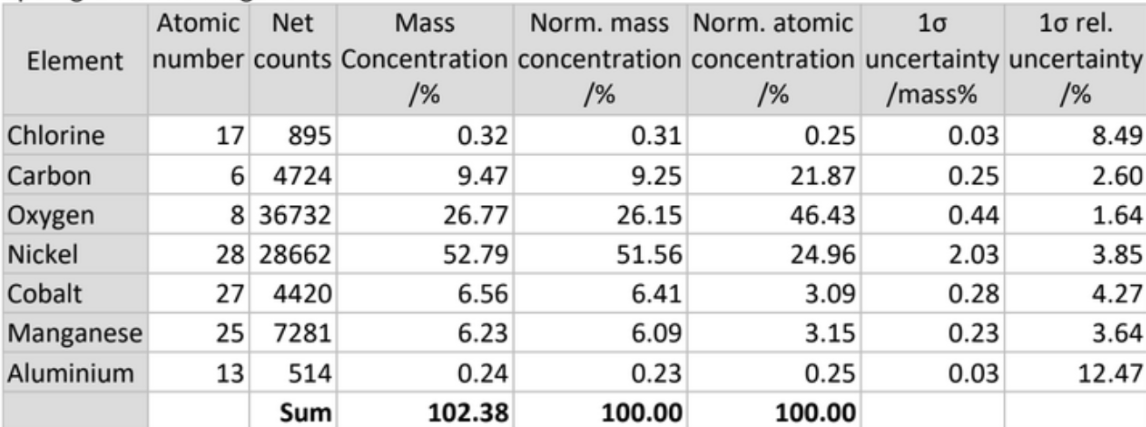
\includegraphics[width=0.8\textwidth]{tabl.png}
  \caption{EDX Composition of NMC 811 4:6 sample.}
  \label{tabl}
\end{figure}
\subsubsection{Size and shape analysis}
The size of the NMC particles being too small (\(<1\) micrometer) significantly affected 
the quality of the SEM images. The automatic calculation 
of the software ImageJ by Fiji relies on distinct boundaries 
and clear contrast to detect and measure particles, which the
 blurry images could not provide. The high sharpness required
  to capture such fine details introduced challenges in
   obtaining clear and distinguishable images. Consequently, 
   the pictures appear blurry, making it difficult for the 
   software to accurately identify and measure individual 
   particle boundaries. Due to this limitation, the particle
    diameter distribution was calculated manually using Fiji,
     by measuring the length of 200 particles and to 
     consequently create a distribution on MATLAB. 
     This method gives an estimation of this size 
     distribution, although the precision might not
      be as high as the automatic one. The 4:6 was too blurry
       to be measured even manually, as the particles were 
       very small. The results can be seen on figure \ref{distributions}\\
      \begin{figure}[H]
        \centering
        \begin{minipage}{0.8\textwidth}
          \centering
          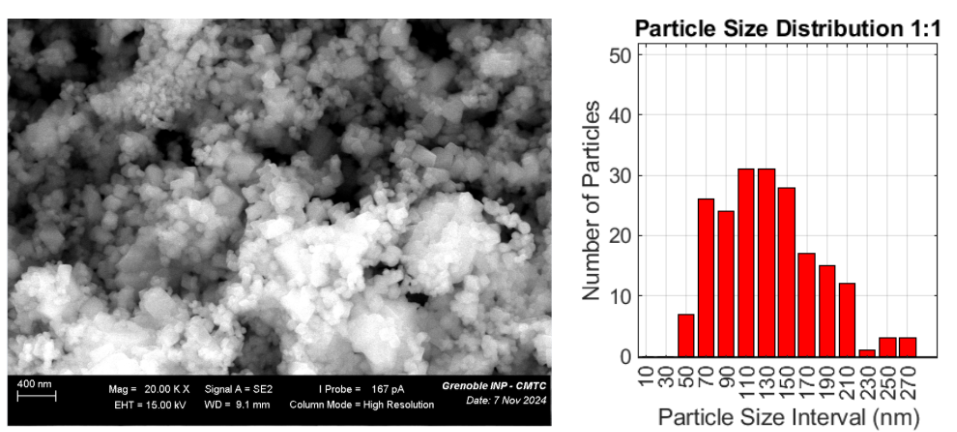
\includegraphics[width=\textwidth]{oneone.png}
          
        \end{minipage}
        \vfill
        \begin{minipage}{0.8\textwidth}
          \centering
          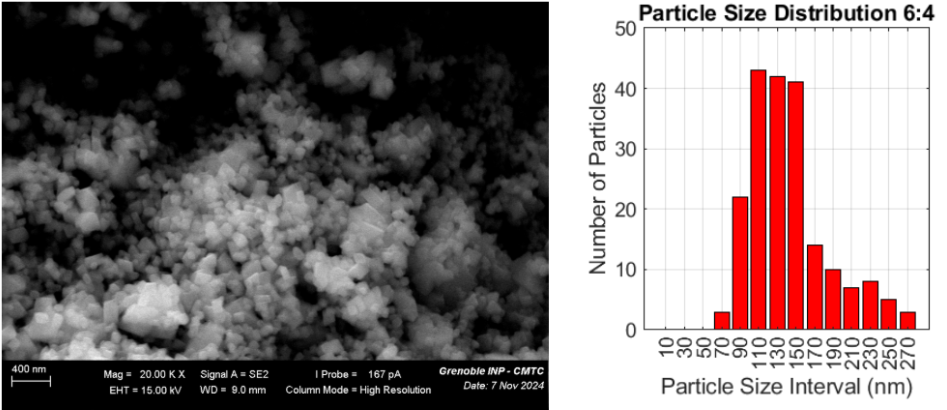
\includegraphics[width=\textwidth]{sixfour.png}
          
        \end{minipage}
        \vfill
        \begin{minipage}{0.8\textwidth}
          \centering
          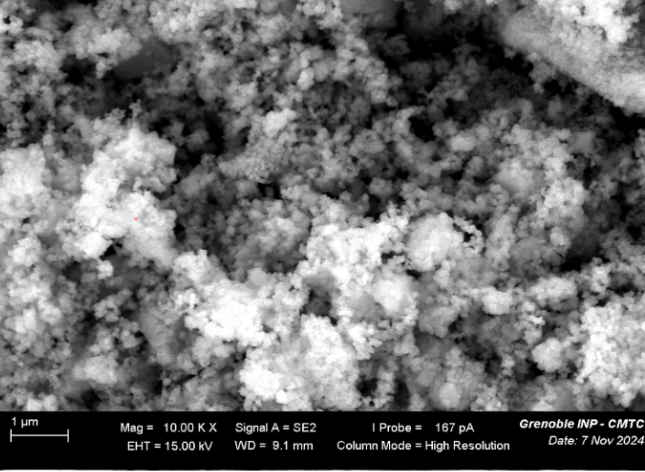
\includegraphics[width=\textwidth]{foursix.png}
          
        \end{minipage}
        \caption{ SEM (washing and annealing without ball-milling) based on \ref{emmanuel} and SEM analysis with FIJI software, ImageJ, distribution made on MATLAB for three different salts proportions (NaCl: KCl).}
\label{distributions}
      \end{figure}

The comparison between the NMC materials with various NaCl:KCl mixtures (1:1 and 6:4) highlights notable differences in particle size, morphology, and degree of aggregation. With the 1:1 mixture, the particle size distribution is relatively distributed with a peak around 130 nm. Concerning the material morphology, its diversity with a mix of rounded and cubic particles suggests a balanced influence of both salts on the crystallization process, leading to well-defined and moderately homogeneous structures. As for the 6:4 mixture (higher NaCl content), it features larger particles with a narrow size distribution, peaking around 150 nm. Moreover, this material displays flatter and more cubic shapes, reflecting NaCl's dominance and its tendency to promote planar crystal growth. On the contrary, the 4:6 mixture (higher KCl content) is characterized by smaller, less-defined, and more rounded particles. It also shows a higher degree of aggregation, with particles forming clusters rather than remaining distinct. These differences indicate that increasing the KCl proportion affects the crystallization dynamics, resulting in less defined shapes and a greater tendency for particles to agglomerate. \\
\begin{table}[H]
  \centering
  \begin{tabular}{|c|c|c|}
    \hline
    \textbf{NaCl:KCl proportion} & \textbf{Size (nm)} & \textbf{Distribution} \\
    \hline
    1:1 & 130 & Homogeneous in shape and sizes \\
    \hline
    6:4 & 150 & Predominance of squared and flat particles \\
    \hline
    4:6 & smaller & Predominance of rounded particles \\
    \hline
  \end{tabular}
  \caption{Particle size and morphology summary for different NaCl:KCl proportions.}
  \label{tab:particle_size_distribution}
\end{table}
The morphology of active particles is a parameter of prime importance in our case, as it directly impacts battery performance. Round particles offer better mechanical stability by reducing stress concentration points, which lowers the risk of cracking and improves long-term durability. Flat particles, with their exposed facets, provide higher specific surface area, enabling faster electrochemical reactions. However, this type of grain is more prone to mechanical and chemical degradation due to stress accumulation at the edges. The choice between these morphologies affected by the NaCl/KCl ratio involves a balance between performance (higher capacity is expected with plate particles) and durability (round particles), depending on the specific application requirements. \\

Based on this theoretical information, a higher capacity is expected for the coin cell with the NMC material prepared with a 6:4 salts ratio, and the lower one should be with the 4:6 salts ratio. Regarding durability, the most durable is expected to be the material prepared with a salts ratio of 4:6, then 1:1 and finally 6:4.\\

By comparing the obtained particle size with those reported in other NMC molten-salt-based synthesis studies, the particles obtained in this work (Figure \ref{distributions}) are the smallest range observed. Jian Zhou et al. used a similar protocol but with a different lithium source \(Li_2CO_3\) instead of LiOH, as employed in this project, and reported 1 to 5 micrometers particles using the same salt-to-NMC ratio. When the salt amount was significantly increased relative to the NMC precursors over 40 times more salt than NMC,they achieved particle sizes of 0.1 micrometers. This ratio, however, greatly exceeds the salt proportion used in this study, highlighting a possible other phenomenon causing the particle's size reduction (at first that something happened differently)\cite{Jian}\cite{shape}.\\

In the case of the other washing protocol (ball milling + washing (BM+W)), the size as well as the morphology of the NMC particles is similar. This observation implies that the additional ball milling step did not affect the particle size, but as these grains are very small, the experiment is  to be done with bigger particle synthesis to see if this assumption remains true.\\
\subsection{Purity analysis by XRD}
The XRD patterns obtained for both ball-milled and not ball-milled series of three samples were 
analyzed using XRD patterns corresponding to a NMC 811 material, a NaCl salt and a KCl salt found in
 literature. The pattern's superposition shows the NMC 811 phase presence, while the salt's patterns
 do not correspond to the peaks obtained (Figure \ref{XRD}). This statement is done for each material, i.e.for
 each salt ratio and each protocol (ball-milled or not). However, the intensity of some NMC 811 peaks do 
not correspond to the synthesized ones. For instance, at around \(2\theta=36^\circ\) and \(38^\circ\), the intensity is respectively
 small and high on the XRD pattern obtained, and the contrary on the NMC pattern reference. This could be due
 to the lack of lithium in the material. In any case, there seems to be a NMC
 811 phase in the material as expected, without salt presence according to the XRD analysis.\cite{mambo}\cite{tango}\\
\begin{figure}[H]
  \centering
  \begin{minipage}{0.48\textwidth}
    \centering
    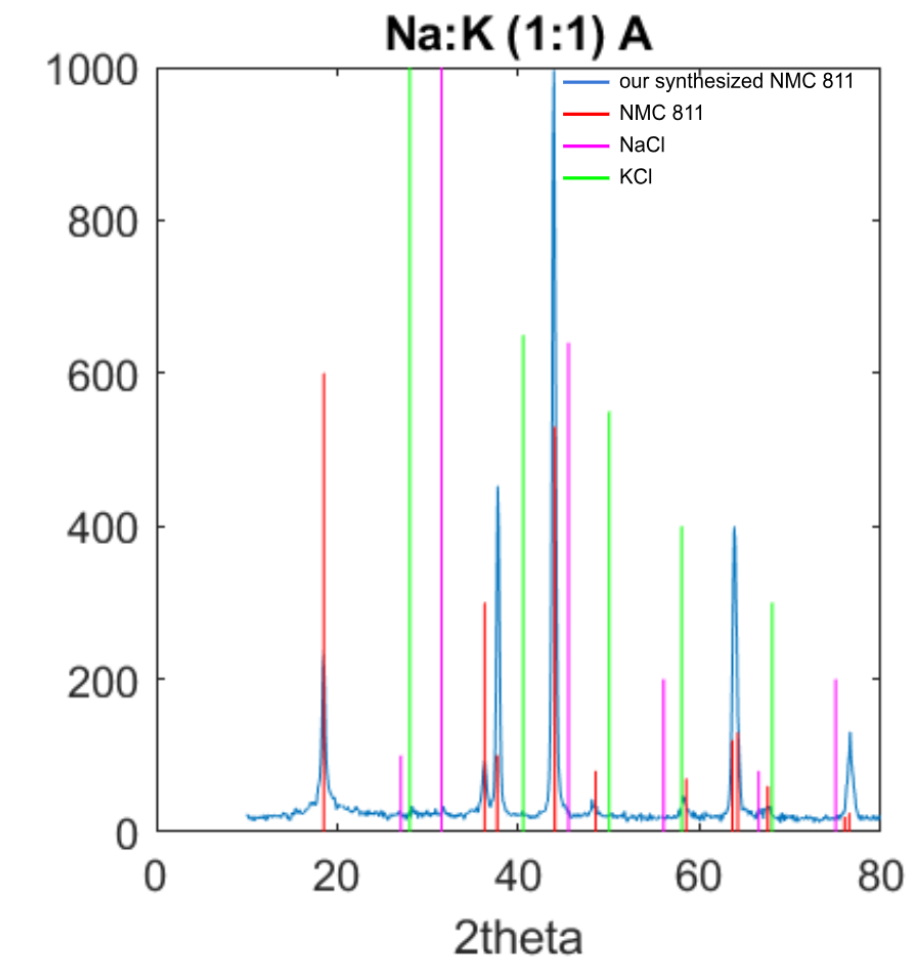
\includegraphics[width=\textwidth]{XRD_A.png}
    \label{fig:output}
  \end{minipage}
  \hfill
  \begin{minipage}{0.48\textwidth}
    \centering
    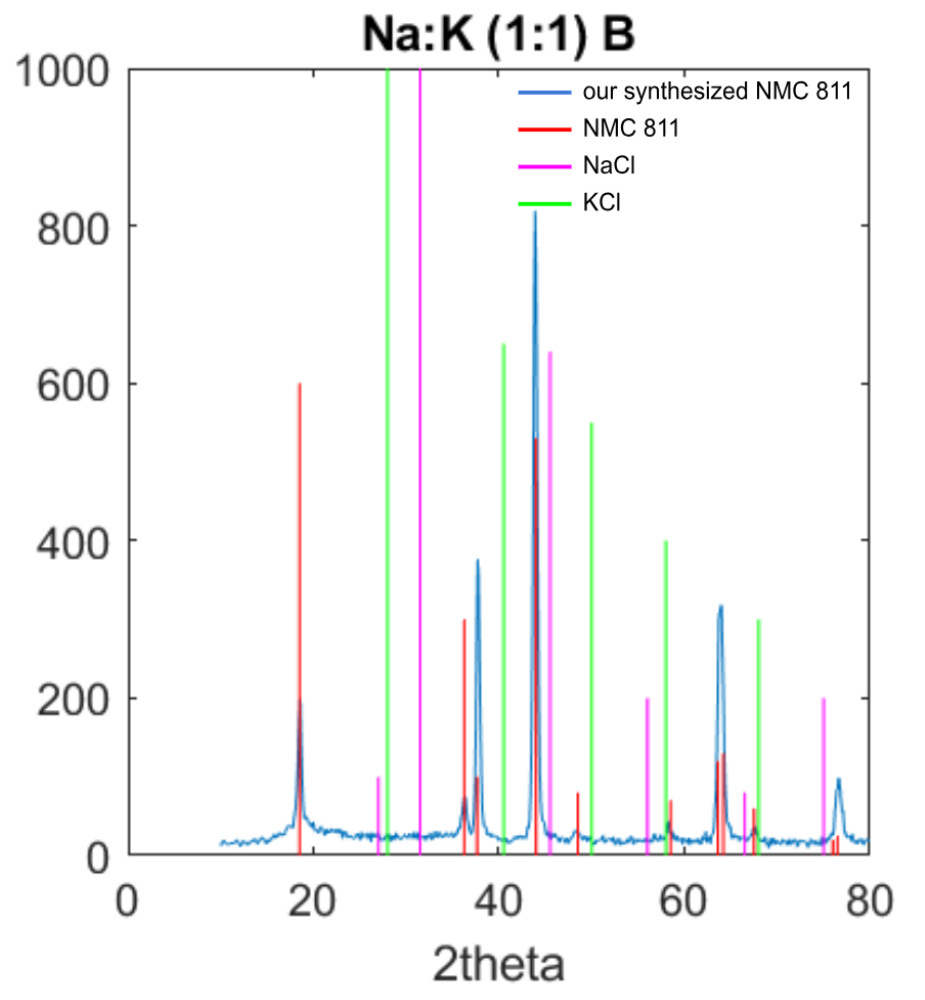
\includegraphics[width=\textwidth]{XRD_B.png}
    \label{fig:output3}
  \end{minipage}
  \caption{ XRD patterns plotted on Matlab of the NMC 811 synthesized with a salt ratio of 1:1 where NMC811 [NMC811DRX] (red), NaCl and KCl [KCl] a)no ball-milling before washing, with annealing and b) with ball-milling before washing but no annealing}
  \label{XRD}
\end{figure}
\subsubsection {Purity analysis by EDX}
\begin{itemize}
  \item Washed + annealed NMC materials\\
  These samples are washed with water and annealed. According to the SEM picture, the salts have left during the washing step,
   leaving the NMC particles with the correct stoichiometry as expected. However, some remaining salt particles have been observed,
   for instance in the 6:4 sample as displayed by Figure \ref{EDX1}, showing an undesired agglomerate of KCl. The NaCl appears to be well-removed,
   while the KCl is not. Some traces of Cl can be seen in every sample, while the 1:1 seems to contain less of K than the 6:4 and 4:6 samples.
  To see the homogeneity as well as the particles shape and size, see 5.1.2.\\
  \begin{figure}[H]
    \centering
    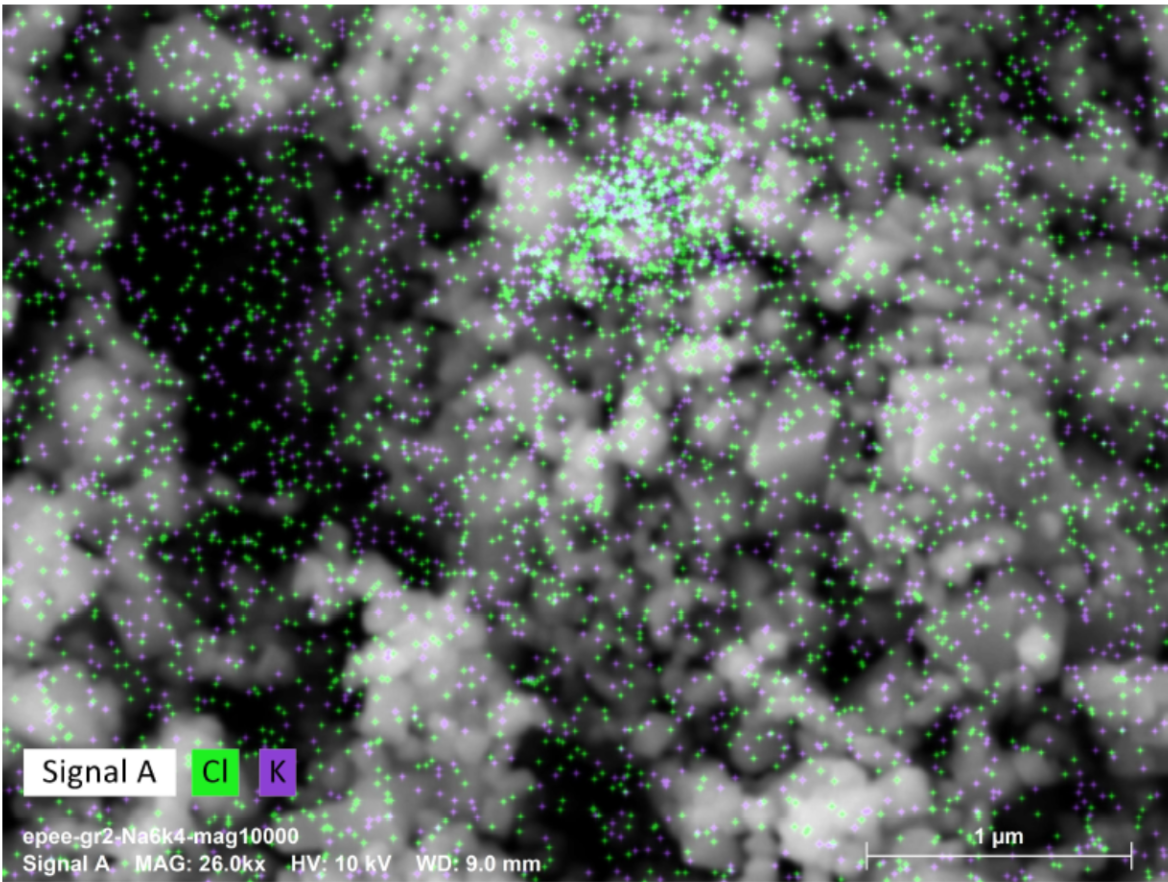
\includegraphics[width=0.8\textwidth]{EDX1.png}
    \caption{SEM picture coupled with EDX mapping of chlorine and potassium in the NMC synthesized with a NaCl:KCl ratio equals to 6:4 after washing and annealing.}
    \label{EDX1}
  \end{figure}
  \item Ball-milled + washed NMC materials\\
  The interest of the additional ball-milling step lies in a
   reduction of the size of some agglomerates that could have been 
  formed during calcination. This second protocol aims to test the ball-milling 
  influence on the particle size and morphology obtained, and also to efficiently 
  remove all the salts in the NMC precursors. The ball-milling first successfully 
  contributes to obtaining a thin powder that is washed and analyzed. According to
   EDX coupled with SEM, there are no significant traces of NaCl and KCl, implying 
  that this step also helps to synthesize a material without any remaining salts. 
  Without ball-milling, the washing could not remove all the NaCl and KCl salts. 
  Moreover, the ball-milling step does not impact the particle size, as the value
   of around 100 nm for the BM+W 1:1 is close to 110nm that was mostly found for 
  the samples without ball-milling. The material obtained thus seems to be better in terms of NMC purity.\\
  \end{itemize}
\subsubsection{Lithium amount in  \({Li(Ni}_{0.8}{Co}_{0.1}{Mn}_{0.1}{)O}_{2}\)}
The ICP results highlight a critical issue in the synthesis protocol.
 Lithium does not appear to be incorporated into the structure (0.37 to 0.42 mole for a NMC mole) 
and is instead recovered in significant quantities -77\% of the initial amount in the washing water.
 However, the ICP analysis confirms that the Ni Mn Co material maintains the correct stoichiometry in each sample
, just as the EDX results. Furthermore the presence of ball milling as well as the last
 annealing step do not seem to affect the amount of Lithium in the final NMC811 material. The concentrations can be seen
 on table \ref{ICP_results} \\
\begin{table}[H]
  \centering
  \begin{tabular}{|c|c|c|c|c|c|}
    \hline
    \textbf{Sample} & \textbf{Li (mol)} & \textbf{Ni (mol)} & \textbf{Mn (mol)} & \textbf{Co (mol)} \\
    \hline
    1:1 (W+A) & 0.37 & 0.80 & 0.10 & 0.10  \\
    \hline
    4:6 (W+A) & 0.38 & 0.80 & 0.10 & 0.10 \\
    \hline
    6:4 (W+A) & 0.39 & 0.80 & 0.10 & 0.10 \\
    \hline
    1:1 (BM+W) & 0.40 & 0.80 & 0.10 & 0.10  \\
    \hline
    4:6 (BM+W) & 0.41 & 0.80 & 0.10 & 0.10  \\
    \hline
    6:4 (BM+W) & 0.42 & 0.80 & 0.10 & 0.10  \\
    \hline
  \end{tabular}
  \caption{ICP results for different samples showing the molar amounts of Li, Ni, Mn, and Co.}
  \label{ICP_results}
\end{table}
This small amount of lithium is very inferior to what was expected for the NMC811 material, hence a possible mal-functioning during electrochemical use in a Li-ion battery. 
The capacity of a cell depends directly on the amount of lithium reversibly inserted and extracted during cycling. 
If only 40\% of the lithium (0.4) is initially available  for cycling, the capacity is limited and decreases starting from
 the very first cycle. The main cause of this effect is due to the cell charging involved in the first step of its test,
 during which all the lithium initially present in the positive electrode (NMC811) is transferred to the negative electrode
 (lithium chip). During this process, a portion of the lithium is consumed to form the Solid Electrolyte Interphase (SEI)
 on the negative electrode. This SEI layer is formed to increase the stability and safety of the cell but causes an irreversible
 loss of lithium during the first charge. Consequently, the capacity of the cell diminishes from its theoretical capacity in the
 first cycle.\cite{capacity}\\

A possible hypothesis to address this issue could involve discharging first to lithiate the NMC811. However, this approach
 would only be feasible if the structure \({\text{Li(Ni}}_{0.8}{\text{Co}}_{0.1}{\text{Mn}}_{0.1}{\text{)O}}_{2}\)
 is with x not too close to zero. When \(x<1\), the absence of 
sufficient lithium may result from structural instability or the lack of well-defined pathways for lithium insertion, making
 re-lithiation ineffective. \cite{lithiation}

 \subsection{Stepwise analysis from synthesis}
 To discover and understand why the lithium has been washed away with salts in the water. SEM and XRD were done at different steps of the molten-salt based NMC synthesis (with a salt ratio of 1:1).\\
 \subsubsection{Precalcination sample analysis}
 The SEM and EDX reveal the presence of NaCl and KCl salts in the precursor NMC material,
 in agglomerate form. This is shown by Figure \ref{precalc} a) and b), as the EDX mapping of sodium
, potassium and chlorine highlight the salt particles. With a size of a few tens of micrometers,
 they are bigger than the other particles observed. As these samples have not been calcinated yet,
 the salts have not melted and the NMC grains are not formed. Particles of Nickel,
 Manganese and Cobalt are indeed not well-dispersed inside the volume as the EDX mappings of Figure
 \ref{precalc} c) and d) display. Small agglomerates of cobalt can be observed, without a lot of nickel. \\
\begin{figure}[H]
  \centering
  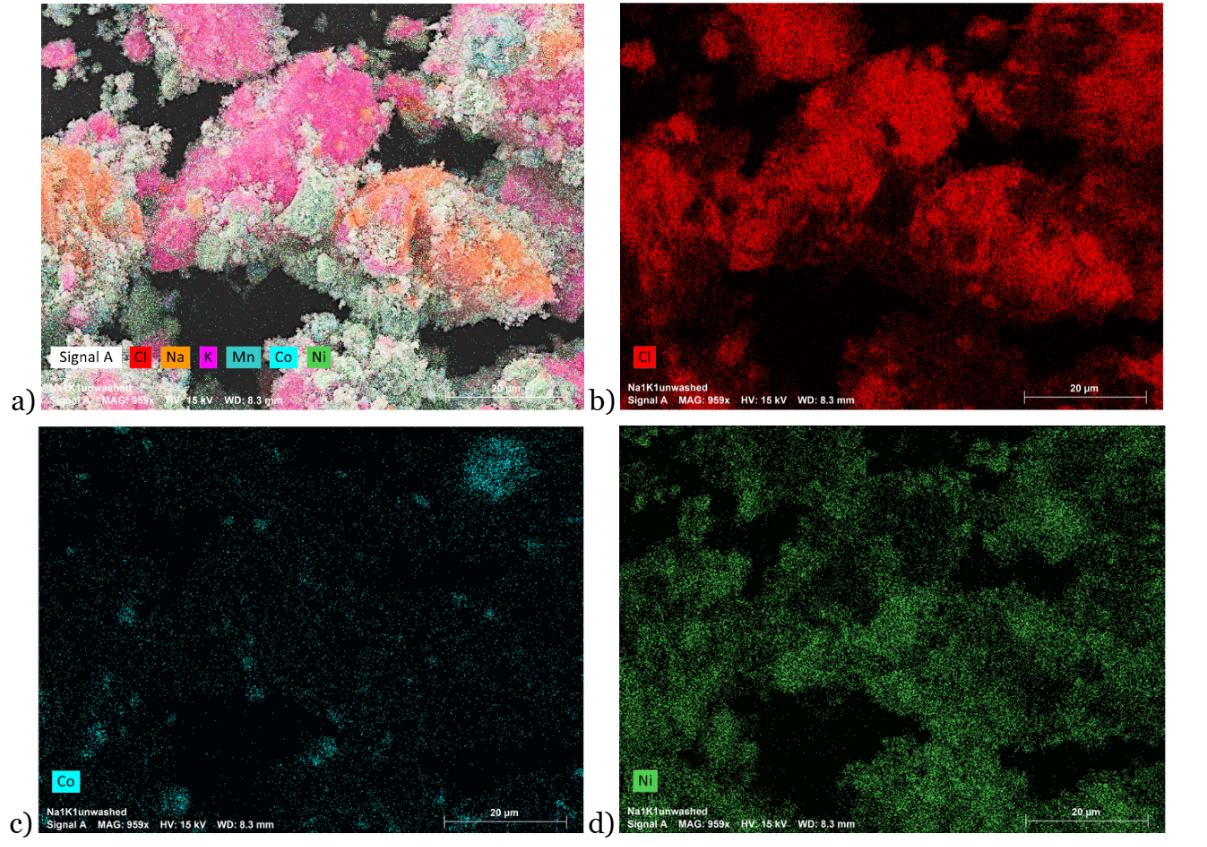
\includegraphics[width=0.8\textwidth]{precalc.png}
  \caption{a) SEM coupled with EDX picture and EDX mappings of b) chlorine, c) cobalt, d) nickel in the NMC precursor synthesized with a NaCl:KCl ratio equals to 1:1 after pre-calcination}
  \label{precalc}
\end{figure}
Concerning the proportions of each species in the material, the 1:1 salt ratio is respected
 in the corresponding NMC sample, according to the EDX results. The normalized atomic concentration
 is indeed 4.82\% for Na and 4.68\% for K, which are very close values, while the chloride one is 10.02\%.
 As for NMC ratio, the atomic concentration is 7.41\% of nickel, 0.97\% of manganese and 0.60\% of cobalt.
 It respects the ratio of the NMC811, as the quantity of Mn and Co are similar, while the Ni quantity
 is approximately 8 times superior The Co concentration is a bit low here, but it is not really
 representative of the real Co as this element is not well-dispersed in the material. A broader 
picture should provide a more appropriate Co concentration value.\\
\subsubsection{Calcination sample analysis}
The 1:1 sample was analyzed with SEM and EDX techniques after calcination. The material has not been washed yet,
 hence KCl and NaCl particles' presence. They are dispersed in the sample. Concerning the NMC, the ratio is 811 
as it should and it is agglomerated on the salt particle: the normalized atomic concentration is 32.98\% Ni, 
3.51\% Co and 4.34\% Mn according to the EDX (Figure \ref{calc} a)). The role of the calcination step is highlighted by
 comparing these results to the ones for the pre-calcined 1:1 sample. Contrary to the agglomerates of Ni, Mn 
and Co we had, after calcination the particles are more dispersed in the materials. The calcination helps to 
melt the salts and to form the NMC811 particles. The shape of the salt particles have changed according to the 
SEM results: the size is still around some micrometers (the SEM picture shows a particle of around ten micrometers,
 which is a bit smaller as in the pre-calcined sample but a more global view should be done over the material to assert
 the salt particles shrink during calcination), but they seem to be a bit sharper after than before the  calcination step.\\

\begin{figure}[H]
  \centering
  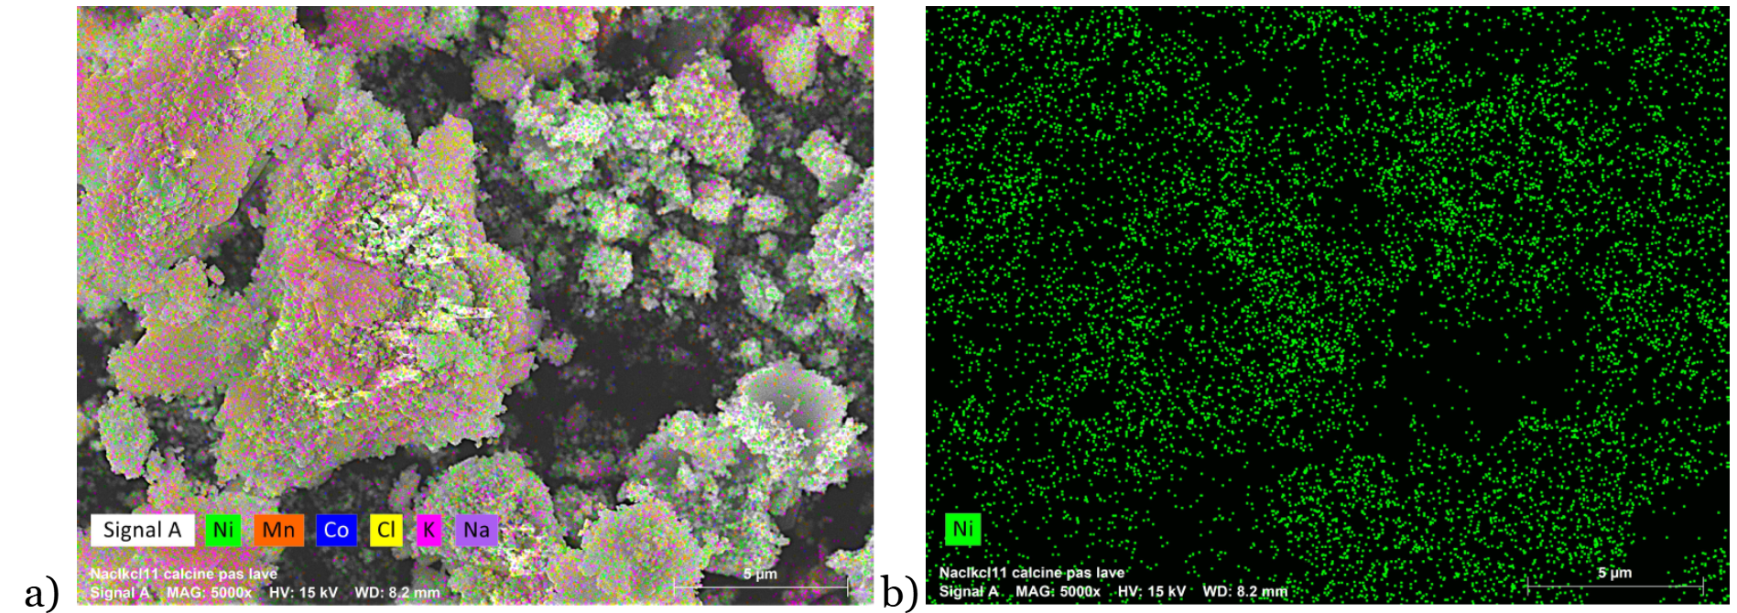
\includegraphics[width=0.8\textwidth]{calc.png}
  \caption{SEM coupled with EDX picture and b) EDX mappings of nickel in the NMC synthetized with a NaCl:KCl ratio equals to 1:1 after calcination}
  \label{calc}
\end{figure}
The particle size was measured and compared before and after the calcination step using distributions. 
According to Figure \ref{distrom}, the NMC particle size is initially mainly around 80 nm while after calcination 
it is mainly between 80 and 100 nm. The sintering enabled a small particle growth, although the size 
measurement was very approximate for the sample before calcination, as the SEM picture was not zoomed in enough. 
These results should thus be considered carefully.\\
\begin{figure}[H]
  \centering
  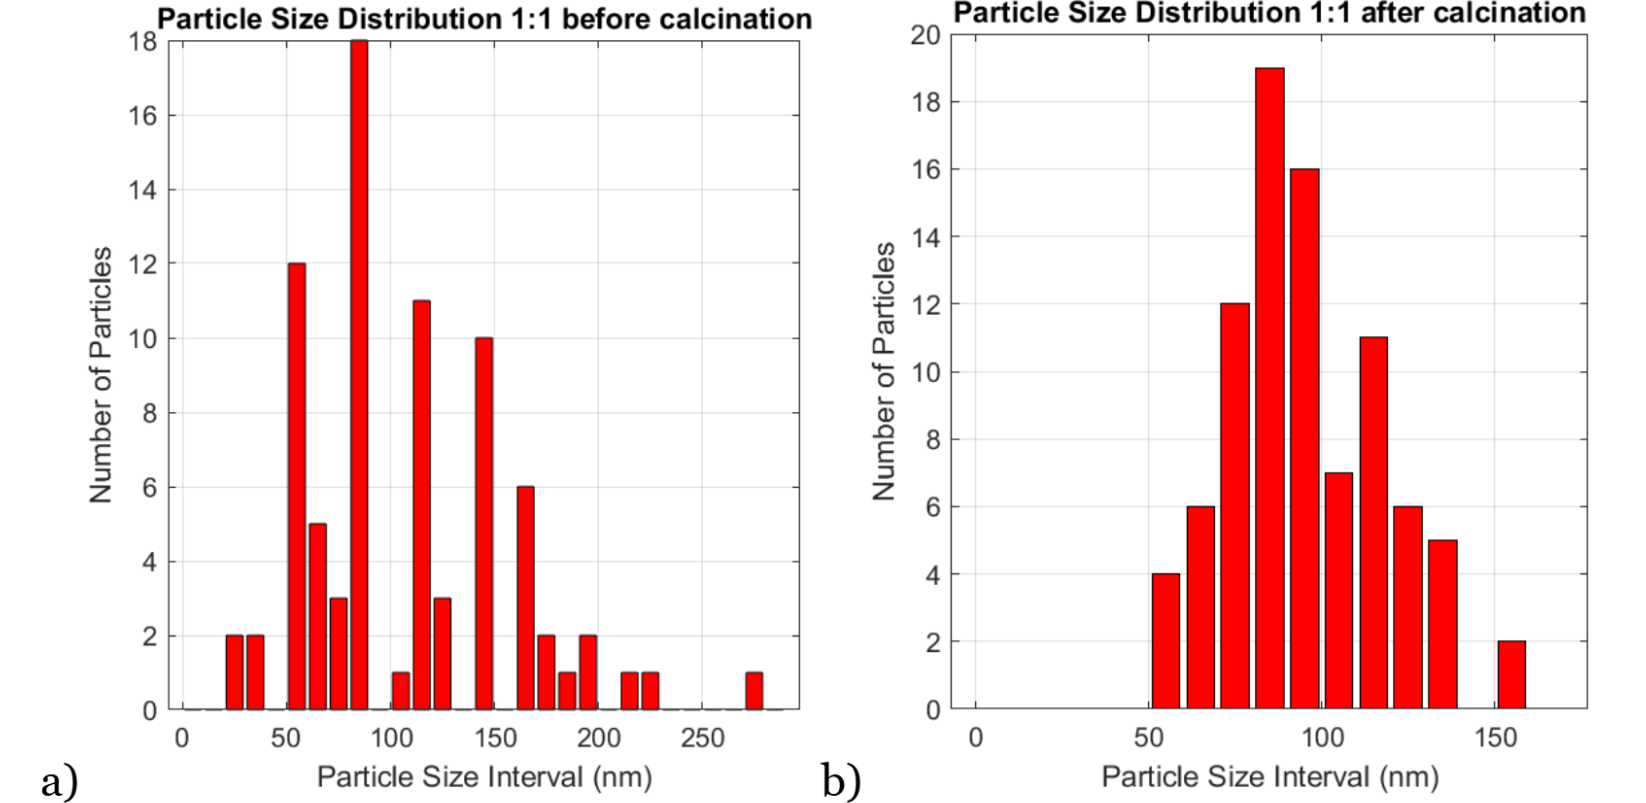
\includegraphics[width=0.8\textwidth]{distrom.png}
  \caption{Size distribution of NMC particles in a material prepared with a NaCl:KCl ratio of 1:1 a) between precalcination and calcination, b) after calcination (see Appendix for the SEM pictures studied) }
  \label{distrom}
\end{figure}
During the calcination, Ostwald ripening does not seem to happen in these conditions: with this salt,
 at \(800^\circ C\) and during 12 hours. The size of particles should have significantly increased during the
 process.\cite{B}\cite{shape}.\\ 
In order to see how every parameter influences the ripening of particles, a 
“experimental plan” can be done with the previously mentioned parameters (Sintering temperature, time and salt amount).  
Moreover, having a NMC particle size around 100 nm provides a higher discharge capacity at different cycling rates 
(C/25, C/10 and C/5) than with bigger particle sizes, such as 1 µm or 10µm. However, the specific area being higher
 for small particles, the latter are more quickly deteriorated while cycling the battery.\cite{Jian} 
The materials prepared are then interesting in terms of discharge capacity, while their durability is expected to be low. \\  

\subsubsection{XRD comparison of precalcination and calcination}
The absence of lithium in the NMC811 samples led to the search for LiCl in the material as a potential explanation.
Precalcined and calcined samples were analyzed to understand the phase formation of NMC811 during calcination. 
In all XRD patterns, the presence of NaCl and KCl was detected, but LiCl was not observed Figure \ref{XRD3}.
 This dismisses the hypothesis that LiCl formed during precalcination and was removed during the washing process. \\
After calcination, the NMC811 phase appears while it was not present before on Figure \ref{XRD4}. This illustrates the transition between carbonate precursors and the NMC811.\\
\begin{figure}[H]
  \centering
  \begin{minipage}{0.7\textwidth}
    \centering
    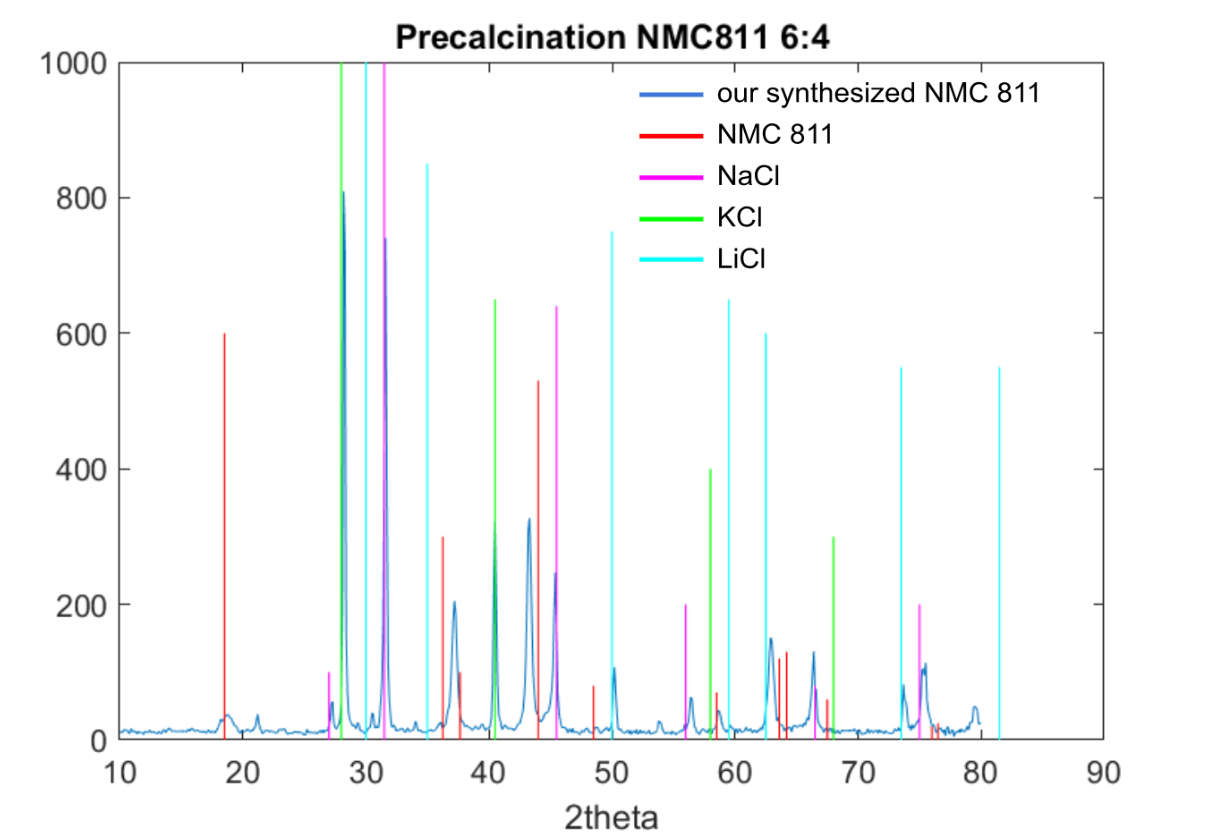
\includegraphics[width=\textwidth]{XRD3.png}
  \caption{XRD patterns after precalcination using NaCl:KCl (6:4) molten salts to synthesize NMC811,  where NMC811 \cite{mambo} (red), NaCl and KCl [KCl], LiCl [LiCl]}
    \label{XRD3}
  \end{minipage}
  \vfill
  \begin{minipage}{0.7\textwidth}
    \centering
    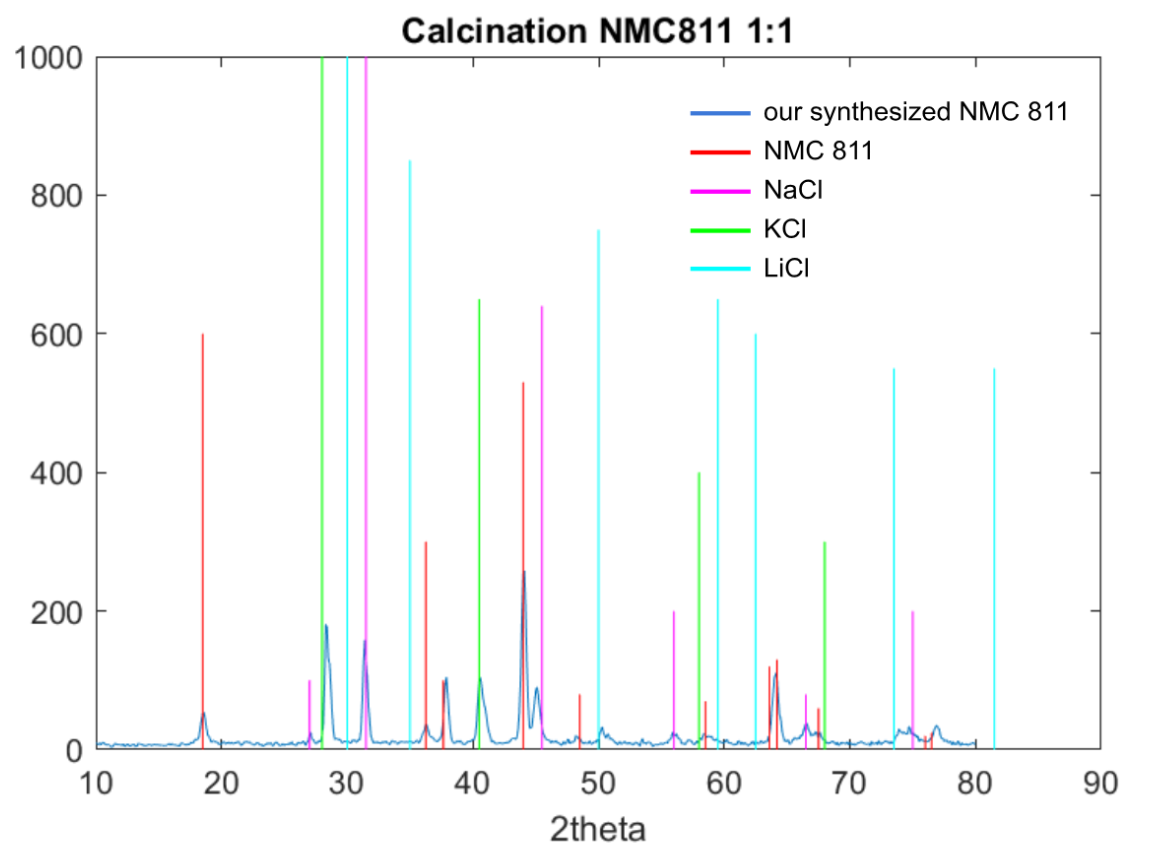
\includegraphics[width=\textwidth]{XRD4.png}
    \label{fig:XRD_calc}
  \end{minipage}
  \caption{XRD patterns after calcination using NaCl:KCl (1:1) molten salts to synthesize NMC811.}
  \label{XRD4}
\end{figure}
\section{Conclusion}




\section{Annexes} 
\begin{figure}[H]
  \centering
  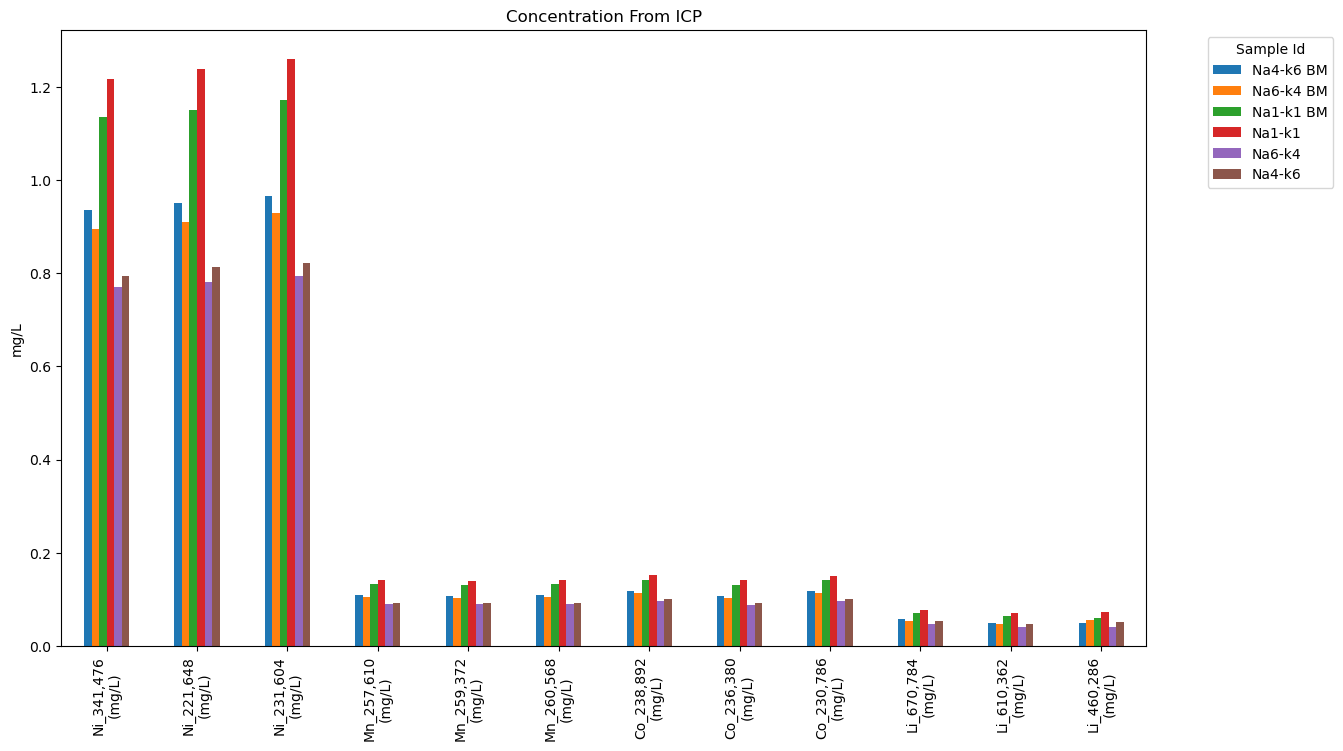
\includegraphics[width=\textwidth]{output.png}
  \caption{Most representative ICP readings for every sample.}
  \label{fig:example_image}
\end{figure}
\begin{figure}[H]
  \centering
  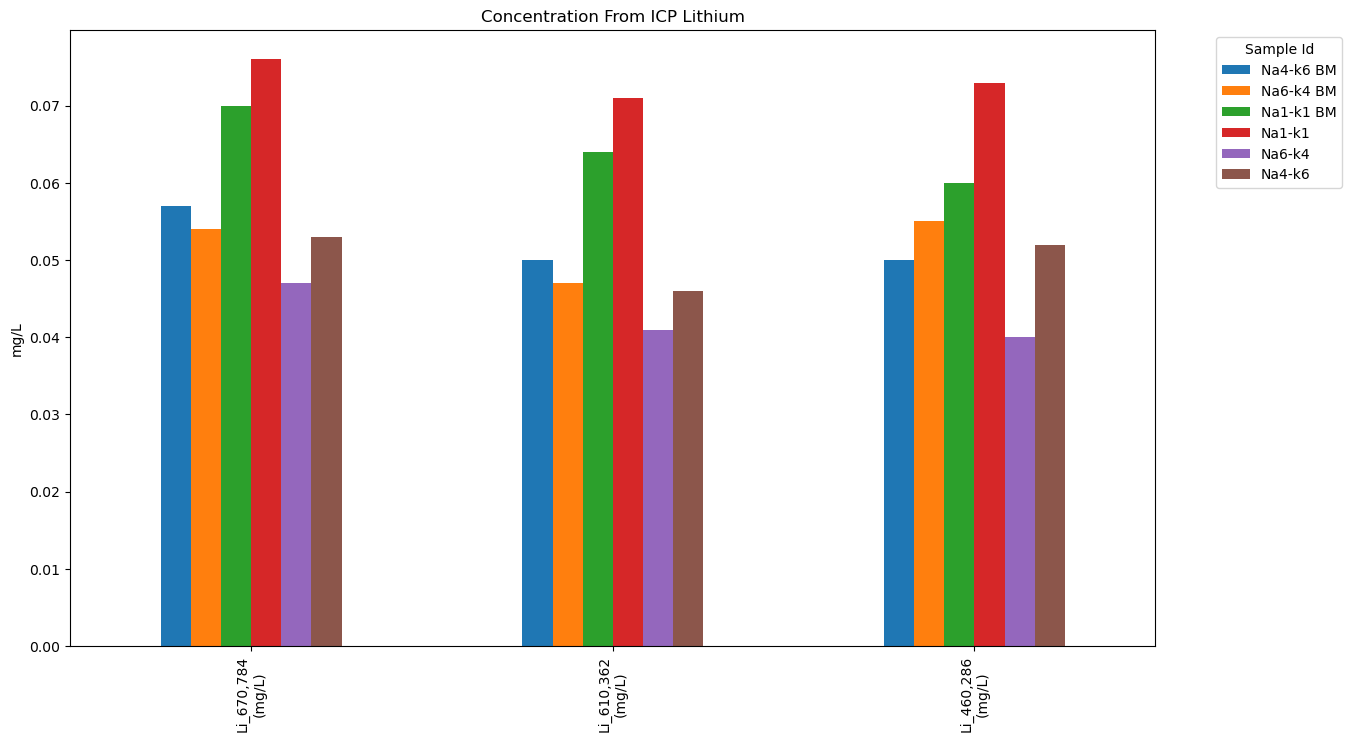
\includegraphics[width=\textwidth]{output3.png}
  \caption{Lithium specific ICP readings.}
  \label{fig:example_image}
\end{figure}
\begin{figure}[H]
  \centering
  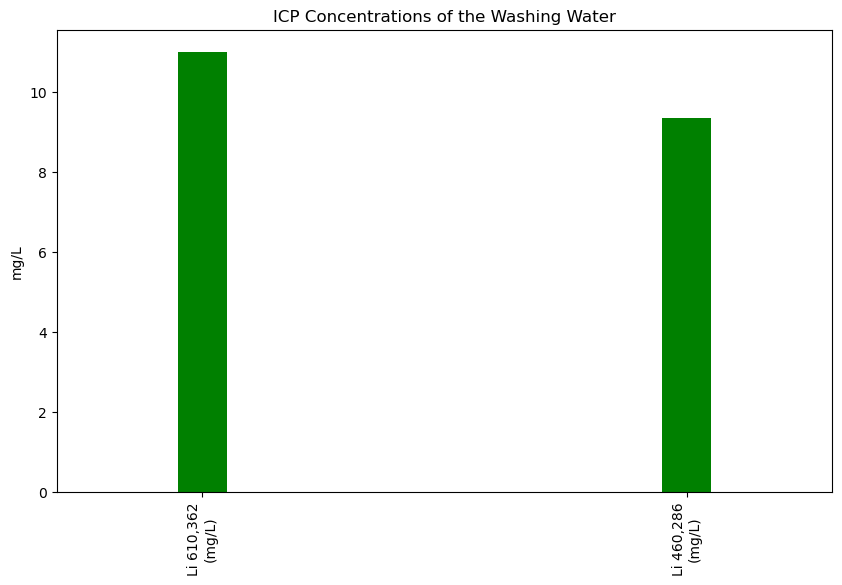
\includegraphics[width=0.8\textwidth]{output2.png}
  \caption{ICP readings for the washing water }
  \label{fig:example_image}
\end{figure}
\newpage
\listoffigures

\listoftables

\bibliographystyle{plain}
\bibliography{Biblio}

\end{document}


